% XeLaTeX can use any Mac OS X font. See the setromanfont command below.
% Input to XeLaTeX is full Unicode, so Unicode characters can be typed directly into the source.

% The next lines tell TeXShop to typeset with xelatex, and to open and save the source with Unicode encoding.

%!TEX TS-program = pdflatex
%change the above line to xelatex if needed
%!TEX encoding = UTF-8 Unicode

%\documentclass[twocolumn, 10pt]{article}
\documentclass[11pt]{article}
\usepackage{geometry}                % See geometry.pdf to learn the layout options. There are lots.
\geometry{letterpaper}                   % ... or a4paper or a5paper or ... 
%\geometry{landscape}                % Activate for for rotated page geometry
\usepackage[parfill]{parskip}    % Activate to begin paragraphs with an empty line rather than an indent
\usepackage{graphicx}
\usepackage{amssymb}
\usepackage{epstopdf}
\usepackage{amsmath}
\usepackage{amsthm}
\usepackage{url}
\usepackage{fancyhdr}
\usepackage{color}
\usepackage{lastpage}
\pagestyle{fancy}
\cfoot{\thepage\ of \pageref{LastPage}}
% Will Robertson's fontspec.sty can be used to simplify font choices.
% To experiment, open /Applications/Font Book to examine the fonts provided on Mac OS X,
% and change "Hoefler Text" to any of these choices.
\usepackage{slashbox} % for table slashbox
%%%%%%%%%%%%%%%% costomed package
\usepackage{listings}\lstset{language = bash}
\usepackage{framed}
\usepackage{setspace}%for double space
%\doublespacing%for double space
%\usepackage{listings}
\newtheorem{theorem}{Theorem}[section]
\newtheorem{lemma}[theorem]{Lemma}
\newtheorem{proposition}[theorem]{Proposition}
\newtheorem{corollary}[theorem]{Corollary}
\theoremstyle{definition}
\newtheorem{definition}[theorem]{Definition}

%%%%%%%%%%%%%%%%
%\usepackage{fontspec,xltxtra,xunicode}
%\defaultfontfeatures{Mapping=tex-text}
%\setromanfont[Mapping=tex-text]{Hoefler Text}
%\setsansfont[Scale=MatchLowercase,Mapping=tex-text]{Gill Sans}
%\setmonofont[Scale=MatchLowercase]{Andale Mono}

\title{Synthetic Data Generation from Topic Models }
\author{}
\date{}                                           % Activate to display a given date or no date

\begin{document}
%\maketitle
%\section{Probabilistic latent semantic indexing (PLSI)}
%PLSI is a statistical latent class model first proposed by Thomas Hofman in \cite{?}. It assumes that a document corpus is generated from a small number of latent topics. Each document has a distribution over topics, and each topic has its own distribution over words. More precisely, suppose there are $n$ documents, $m$ words, and $k$ underlying topics. The model assumes that there exists an $n\times k$ matrix $U$ where each row is a document's distribution over topics, and a $k\times m$ matrix $V$ where each row is a topic's distribution over words. The $i$th document is generated by first picking a document length $d$, then sampling each word from a multinomial distribution given by the $i$th row of $A=UV$. 
%
%We implemented a data generator according to the PLSI model, and tested the performance of various algorithms on the synthetic data. The generator takes parameters
%\begin{itemize}
%	\item $k$, number of latent topics
%	\item $n$, number of documents in the corpus
%	\item $l$, parameter of the poisson distribution determining number of words in a document
%	\item $m$, size of the vocabulary
%	\item $s$, amount of noise per document
%\end{itemize}
%We generate the $n\times k$ matrix $U$ and the $k\times m$ matrix $V$ by choosing each entry uniformly randomly from $[0,1]$, and normalize each row to have $L_1$-norm $1$.
%
%The $i$-th document is then generated as follows:
%\begin{enumerate}
%	\item Determine the length of document $l_i\sim Poisson(l)$
%	\item Determine the number of noise words $s_i\sim Poisson(s)$
%	\item for $d=1,\ldots,l_i-s_i$:\\
%				\hspace*{5 mm} sample a topic $t_{i,d}\sim Multinomial(U_i)$\\
%				\hspace*{5 mm} sample the actual word $w_{i,d}\sim Multinomial(V_{t_{i,d}})$
%	\item for $d=l_i-s_i+1,\ldots l_i$:\\
%				\hspace*{5 mm} sample the $d$-th word $w_{i,d}\sim Uniform(m)$ 
%\end{enumerate}
%The data generator outputs both the generated documents and the model description $U,V$.
%
%
%\section{Latent dirichlet allocation (LDA)}
%LDA is a generative probabilistic model introduced by David Blei et al. in \cite{?}. Like PLSI, it assumes that a document corpus is generated from a finite number of latent topics, that each document has a distribution over topics, and each topic a distribution over words. However, LDA assumes that each distribution is sampled from a dirichlet distribution rather than a random one. 
%
%Our data generator, according to LDA, works much the same way as PLSI. In addition to the parameters for the PLSI model, it has the following:
%\begin{itemize}
%	\item $\alpha$, parameter of the dirichlet distribution from which topic distributions are drawn
%	\item $\beta$, parameter of the dirichlet distribution from which word distributions are drawn
%\end{itemize}
%Here, each row of $U$ is generated by sampling $U_i \sim Dirichlet(\alpha)$, and each row of $V$ is generated by sampling $V_i \sim Dirichlet(\beta)$.
%
%The actual document generation is identical to PLSI.
%
%\section{Recommendations}
%In addition to documents, we generated synthetic data according to PLSI and LDA for recommendations. Instead of documents being a mixture of topics, we assume that we have users who are a mixture of user types. Furthermore, instead of each topic having a distribution over words, each user type has a number of ratings for various items. Formally, suppose there are $n$ users, $M$ is the set of items, and $k$ underlying user types. The models then assume an $n\times k$ matrix $U$ where each row is a user's distribution over user types. However, for the $k\times m$ matrix $V$, each row is no longer a distribution, but instead a list of ratings. The $i$th user is generated by first picking a number of items to rate $d$. Each item is then rated by first sampling from a multinomial distribution given by the $i$th row of $U$ to determine the user type, then by finding the corresponding rating in $V$.
%
%Our generator for recommendations takes the following parameters:
%\begin{itemize}
%	\item $k$, number of latent user types
%	\item $n$, number of users in our system
%	\item $l$, parameter of the poisson distribution determining number of ratings each user has
%	\item $m$, total number of items
%	\item $s$, amount of noise per user
%\end{itemize}
%$U$ is generated according to PLSI or LDA, and $V$ is generated by uniformly at random choosing an integer from $1$ to $5$.
%
%Each user is generated as follows:
%\begin{enumerate}
%	\item Determine the number of items to rate $l_i\sim Poisson(l)$
%	\item Determine the number of noise items $s_i\sim Poisson(s)$
%	\item Select $l_i$ items, $I$, uniformly at random from $1, \ldots, m$
%	\item for each item $d \in I$:\\
%				\hspace*{5 mm} sample a user type $t_{i,d}\sim Multinomial(U_i)$\\
%				\hspace*{5 mm} set the actual rating = $V_{t_{i,d}}$
%	\item Select $s_i$ items, $S$ uniformly at random from $M \setminus I$
%	\item for each item $d \in S$:\\
%				\hspace*{5 mm} sample the $d$-th rating $w_{i,d}\sim Uniform({1,2,3,4,5})$ 
%\end{enumerate}

\setlength\tabcolsep{0.5pt}
\begin{figure*}
	\centering
	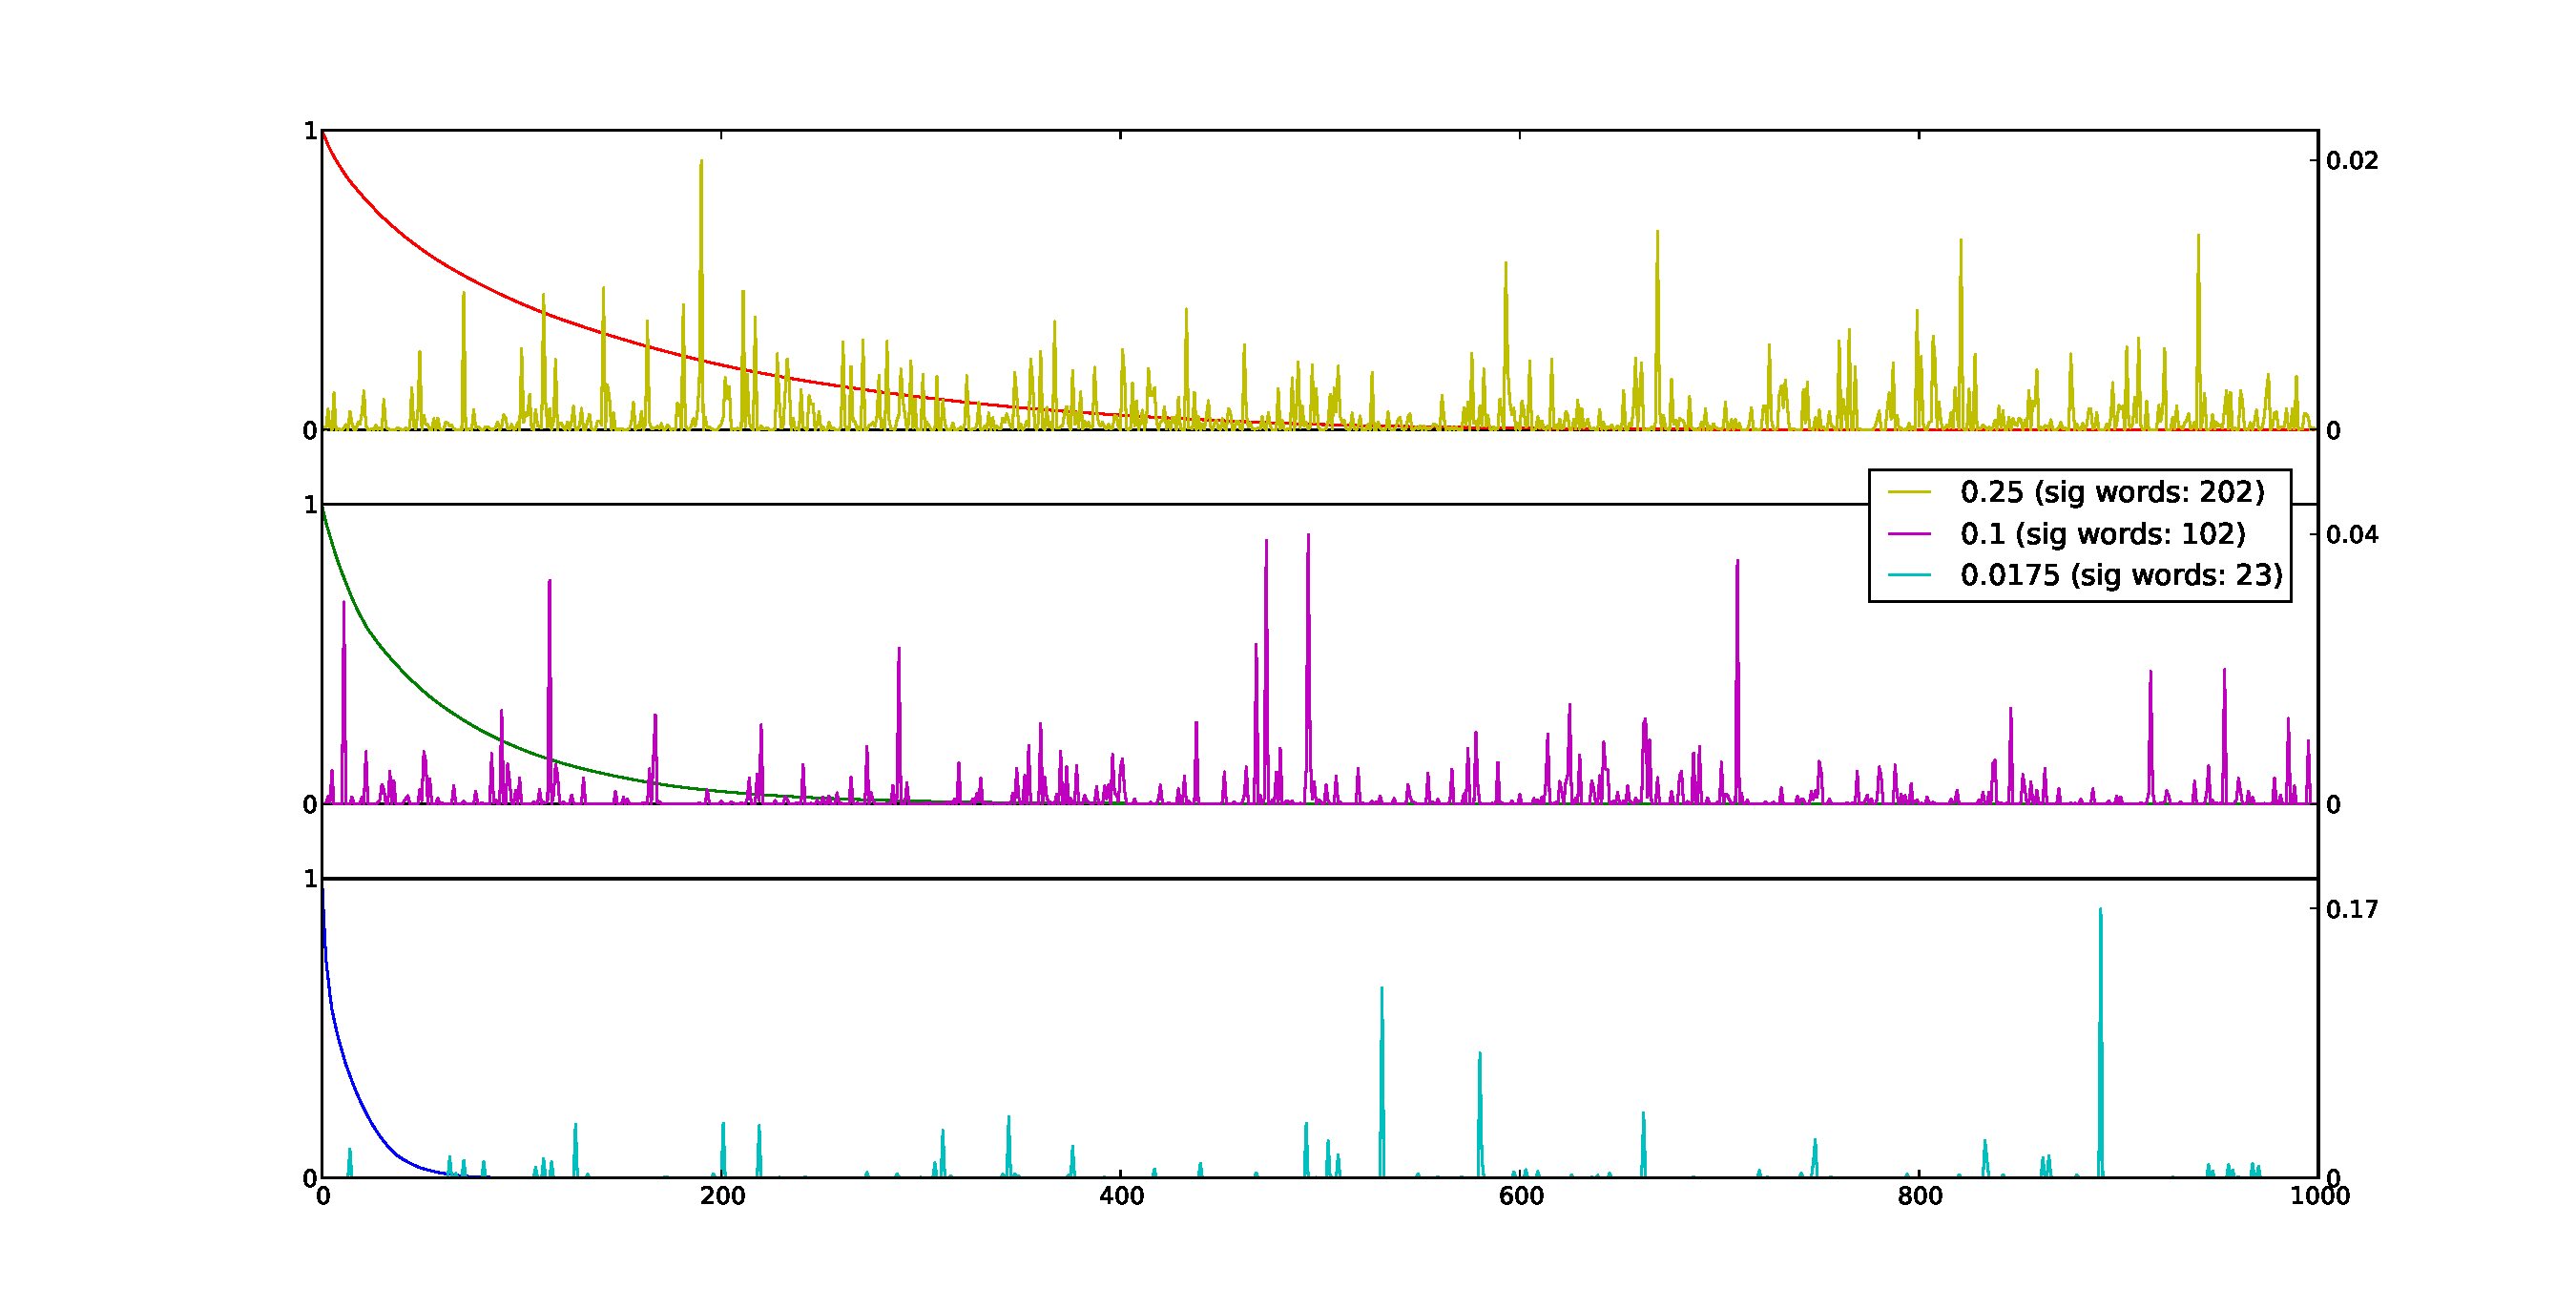
\includegraphics[width=\textwidth]{beta_plots.pdf}
	\caption{A plot of various distributions for different choices of $\beta$. Each distribution is plotted along with its cdf, and has been scaled to span the entire space (refer to the y-axis on the right for the scaling). In general, larger $\beta$ values yield flatter distributions.}
	\label{fig:beta_plots}
\end{figure*} 
\setlength\tabcolsep{6pt}

\input{experiments.tex}

\end{document}
